\documentclass[a4paper, 11pt]{article}
\usepackage[ngerman]{babel}
\usepackage{amsmath}
\usepackage{listings}
\usepackage{pgfplots}
\usepackage{graphicx}
\pgfplotsset{compat=1.9}
\usepackage{tikz}
\author{Lukas Hofmaier}
\title{Recommender}
\begin{document}

\lstset{basicstyle=\small,
language=Haskell,
stringstyle=ttfamiliy
}

\maketitle

\tableofcontents

\section{Recommender-Problem}
\label{sec:problem}

Konsumenten werden heute in vielen Bereichen mit einer un"uberschaubaren Anzahl an Kaufm"oglichkeiten konfrontiert. In einem Webshop f"ur B"ucher oder Filme ist es es f"ur den Konsumenten beispielsweise schwierig, alle Artikel im Angebot anzuschauen und aufgrund dieser Evaluation die besten Artikel auszuw"ahlen. Beim Recommender-Problem geht es darum aus einer Mengen von Artikel (Items) ein sortierte Liste mit den empfehlenswertesten Artikel f"ur einen spezifischen Kunden (User) zu erstellen. Recommender kommen vorallem dort zum Einsatz, wo pers"onlicher Geschmack bei der Bewertung von Artikel eine wichtige Rolle spielt.

Ein Recommendersystem kann eine Bewertung absch"atzen (vorhersagen), die ein bestimmter User und einem bestimmtes Item gibt. Recommender berechnen die Bewertungen f"ur Items die der User noch nicht gesehen hat. Die Items mit den besten Bewertungen werden dem User empfohlen.

Recommendersysteme werden vorallem im e-Commerce eingesetzt. Man kann sie aber auch dazu verwenden um unwichtige Informationen von wichtigen zu trennen.

In nachfolgenden Text wird haupts"achlich von User und Items gesprochen. 

\begin{description}
\item[User] User sind die Konsumenten oder f"ur die eine Empfehlung erstellt werden soll. 
User haben Preferencen und bewerten Items aufgrund des pers"onlichen Geschmacks. 
\item[Item] 
Items k"onnen Artikel, Filme, B"ucher, Dokumente e.t.c sein. Items werden den Usern empfohlen.
\end{description}

Der aktive User bezeichnet den User, f"ur den Empfehlungen erstellt werden soll.

\subsection{Strategien}
\label{sec:strategies}

Es gibt zwei unterschiedliche Strategien f"ur Recommendersysteme: Content filtering und collaborative Filtering. 

\subsubsection{Content based Filtering}
\label{sec:contentbased}

Bei Content based Filtering wird zu jedem Artikel und zu jedem User ein Profile erstellt. Dieses Profile enth"alt Informationen "uber die Eigenschaften von User und Item. Beispielsweise k"onnte man alle angebotenen Filme nach ihrer Genrezugeh"origkeit bewerten. Ein Film hat beispielsweise einen Action und einen Romantikanteil. User k"onnen angeben, ob sie lieber Action oder Romantik m"ogen. Content based Filtering sucht dann Filme, die am besten mit dem Userprofile matchen. Die Schwierigkeit an Content based Filtering ist das Erfassen von Daten zu jedem Item und zu jedem User. Jemand muss jeden Artikel im Angebot nach seinem Content bewerten.

\subsection{Collaborative Filtering}
\label{sec:collaborativefiltering}

Collaborative Filtering ist eine weitere M"oglichkeit das Re\-commender-Prob\-lem zu l"osen. Bei Collaborative Filtering wird das Verhalten von User in der Vergangenheit analisiert. Dabei werden Bewertungen oder Transaktionen angeschaut. Der Inhalt der Artikel ist egal. Da diese Strategie unab"angig vom Inhalt ist kann sie f"ur jedes beliebige Recommendersystem eingesetzt werden. Es kann also im e-Commerce sowie auch im Information Filtering eingesetzt werden.  Es wird vielen Webshops erfolgreich eingesetzt \cite{sarwar01}. 

Ziel des Collaborative Filtering ist es einem User neue Items oder f"ur ein bestimmtes Item und einen bestimmten User eine Bewertung vorauszusagen. Typischweise gibt es eine Menge von $m$ Usern  $\mathnormal{U}$ und eine Menge von $ \mathnormal{I} $ Items. Jeder User $\mathnormal{u}$ hat eine Liste $\mathnormal{I_u}$ von Items, welche er bewertet hat. Diese Bewertung wird meisten als numerischer Wert in einem Intervall ausgedr"uckt. Bei Filmen hat es sich zum beispiel durchgesetzt das man eine Zahl zwischen 1 und 5 angibt, wobei die 5 eine gute Bewertung repr"asentiert. Diese Bewertungen werden von den User explizit eingegeben oder sie werden zum beispiel vom Kaufverhalten abgeleitet.

Man kann zwei Resultate von Collaborative Filtering unterscheiden.

\begin{description}
\item[Prediction] Das System berechnet eine wahrscheinliche Vorhersage $P_{u,i}$ f"ur eine Bewertung von Item i und User u
\item[Empfehlung] Das System gibt eine Liste von $N$ Items zur"uck, die Items in der Liste hat der user noch nicht bewertet und das System hat die h"ochsten Bewertungen f"ur den aktiven User berechnet.
\end{description}

\begin{figure}[h]
  \centering
      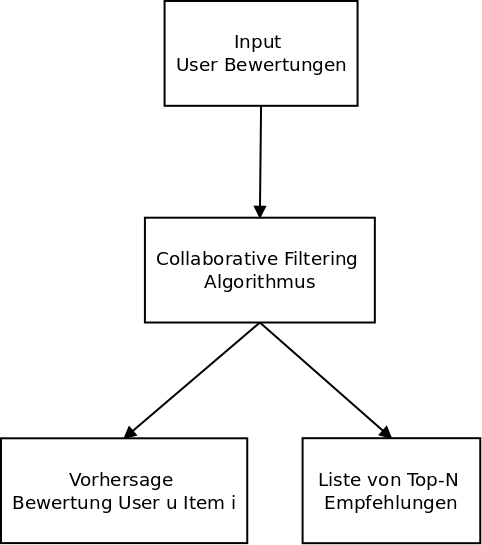
\includegraphics[width=0.5\textwidth]{cf}
  \caption{Collaborative Filtering Prozess}
\end{figure}

Collaborative Filtering kann weiter in zwei unterschiedliche Methoden aufgeteilt werden:

Bei Neighboorhood Methoden werden f"ur jeden User "ahnliche User gesucht. Es wird eine Nachbarschaft mit "ahnlichen User erstellt.

"Ahnlichkeit wird aufgrund von gemeinsam bewerteten Item berechnet. Wenn zwei User f"ur mehrere Items die selben Bewertungen vergeben, sind sie sich "ahnlich. Sie haben einen "ahnlichke Geschmack.

Einem User werden diejenigen Items empfohlen, die er noch nicht kennt und die einge hohe Bewertung von "ahnlichen Usern erhalten haben.

 M"ochte man das Rating von einem User f"ur ein bestimmtes Item ab\-sch"atz\-en, schaut man, ob User in der Nachbarschaft das Item bereits bewertet haben. Aufgrund der "Ahnlickeit und den vorhandenen Ratings berechnet man das Rating das der User f"ur dieses Item abgeben w"urde.


\subsection{Herausforderungen}
\label{sec:challenges}

Bei der Implementierung von Recommendersystemen ergeben sich zwei Herausforderunge.

\begin{description}
\item[Genauigkeit] Die Differenz der Empfehlungen die das Recommendersystem macht sollen so wenig wie m"oglich von der tats"achlichen Bewertung abweichen.
\item[Skalierbarkeit] 
Collaborative Filtering muss f"ur Millionen User und Items m"oglich sein. Die Technik soll also f"ur grosse Datenmengen skalieren.
\item[Sparsity] F"ur eine grosse Menge an Items gibt es in der Regel nur eine kleine Anzahl an Items die ein User auch bewertet hat. Wenn sich keine gemeinsamen Items zwischen den Usern finden k"onnen auch keine Nachbarschaften gebildet werden.
\end{description}


\section{Unpers"onliche Empfehlungtechniken}
\label{sec:simple}

Um einem User Items zu empfehlen werden oft einfache Statistiken berechnet. Diese Methoden sind unpers"onlich. Das heisst die Top-N Empfehlungen sind nicht vom personlichen Geschmack von $u$ abh"angig. Jeder User erh"alt die selben Empfehlungen. 

Diese Technik wird in vielen Bereichen angewendet. Restaurantf"uhrer oder Filmkritikwebseiten erstellen oft Ranglisten, welche Restaurants oder Filme von allen Usern im Durchschnitt am besten bewertet werden. Items mit den h"ochsten Durchschnittswerten, werden dem User empfohlen.

Die einfachste Methode eine unbekannte Bewertung abzusch"atzen ist den Durschnitt aller Bewertungen zu berechnen.

\begin{equation}
  \label{eq:avg}
  b_{u,i} = \mu
\end{equation}

Diese Methode kann noch erweitert werden, indem man die durchschnittliche Abweichung aller Bewertungen von $b_u$ und die durschnittliche Abweichung $bi$ von Item $I$ ber"ucksichtigt \cite{jannach11}.

\begin{equation}
  \label{eq:bui}
  b_{u,i} = \mu + b_u + b_i
\end{equation}

wobei

\begin{equation}
  b_u = \frac{1}{|I_i|}\sum_{i \in I_u}(r_{u,i} - \mu)
\end{equation}

und 

\begin{equation}
  \label{eq:bi}
  b_i = \frac{1}{|U_i|}\sum_{u \in U_i}(r_{u,i} - b_u - \mu)
\end{equation}

Nach folgend bezeichnet $u$ den aktiven User und $i$ das Item, f"ur das man eine Vorhersage der Bewertung haben m"ochte. $b_ui$ bezeichnet die Absch"atzung f"ur die Bewertung von User $u$ f"ur Item $i$.

\begin{equation}
  \label{eq:baseline}
  b_{u,i} = \mu + b_u + b_i
\end{equation}

\begin{lstlisting}[caption=Baseline predictor, label=lst:baseline]
bui :: User -> Item -> Double
bui u i = mu + bu + bi
  where mu = avg allratings
        bu = computebu u
        bi = computebu i

computebu :: User -> Double
computebu u = sum lookup u usermap

computebi :: Item -> Double
computebi i = sum lookup u itemmap
\end{lstlisting}


\section{User-based collaborative filtering}

Die Technik user-based collaborative filtering ist auch als k-NN (nearest-neighbor) oder Memory-based collaborative filtering bekannt. Der GroupLens Usenet Articel Recommender verwendete als einer der ersten Recommender Systeme User-based collaborative Filtering. Ringo Musice Recommender und der Bell Core video Recommender verwenden auch user-based CF .

User-base collaborative filtering kann in zwei Schritte aufgeteilt werden. 

\begin{enumerate}
\item Nachbarschaft erstellen
\item Aufgrund der Nachbarschaft 
\end{enumerate}

User base filtering sucht nach User, die "ahnlich sind. Eine Nachbarschaft besteht aus einem Subset von $ \mathnormal{U} $ Usern $N$, die die h"ochste "Ahnlichkeit aufweisen. Um die Nachbarschaft zu erstellen wird der aktive User mit allen anderen Usern verglichen. Zu jedem Paar wird ein Wert f"ur die "Ahnlichkeit berechnet.

Bespielsweise m"ochte man die Bewertung von User Peter f"ur den Film "Titanic", den Peter noch nicht bewertet hat, vorhersagen. Man sucht nach anderen Usern die Filme "ahnlich bewerten wie Peter. Dazu analisiert man Filme die Peter und andere User bewertet haben. Um die gesuchte Sch"atzung zu erhalten eribt sich aus den gewichteten Wertungen dieser "ahnlichen User. Die Bewertung f"ur Titanic con Usern die Peter sehr "ahnlich sind haben ein gr"osseres Gewicht als die Bewertungen von Usern die Peter unahnlich sind oder sie werden gar nicht ber"ucksichtigt.

Die Technik um "ahnliche User zu finden heisst kNN (k neirest neighbors). 

\subsection{"Ahnlichkeit}

Dieser Abschnitt beschreibt, wie die "Ahnlichkeit zwischen zwei User berechnet wird. 

Es gibt mehrere M"oglichkeiten die "Ahnlichkeit zwischen zwei User zu evaluieren. F"ur die Distanz oder die "Ahnlichkeit gibt es verschiedene Metriken. 

Es ist nur m"oglich die "Ahnlichkeit zwischen 2 User zu berechnen, wenn es ein Subset der Items gibt, die beide User bewertet haben. Wenn dieses Subset leer ist, k"onnen die nachfolgenden Methoden nicht angewendet werden. Der Recommender wurde so implementiert, dass User die keine gemeinsamen Items haben als un"ahnlich bewertet werden.

Wenn es keinen User gibt, der das selbe Item bewertet hat, ist der Korrelationskoeffizient -1.
Die Pearson Similarity ber"ucksichtigt nur gemeinsam geratete Daten.
Was passiert wenn zwei User ein einziges gemeinsames Item haben und dieses gleich bewerten?

\subsubsection{Pearson Korrelation}
\label{sec:pearsoncorrelation}

Um zwei User miteinander zu vergleichen, kann die Pearson Similarity eingesetzt werden.

Wenn man zwei User mit dem Pearson Korrelationskoeffizient vergleichen m"ochte, muss man zuerst alle Items finden die beide User bewertet haben. Wenn die beiden User alle gemeinsamen Items gleich bwertet haben, sind sie sich "ahnlich.

Die Pearson Similariy ber"ucksichtig User die Items konstant tiefer bewerten. Wenn man zwei User die mit den Vektoren (1,2,3,4) und (2,3,4,5) dargestellt werden erhalten die maximale "Ahnlichkeit von 1.

\begin{equation}
 sim(u,v) = \frac{cov(X,Y}{\sigma_X \sigma_Y)} = \frac{(r_{u,i} - \bar{r}_u)(r_{v,i} - \bar{r}_v)}{r_{v,i} - \bar{r}_v}    
\end{equation}

Wenn man diese Formel auf den Vergleich von zwei Usern anwendet, kommt folgendes heraus.
\begin{equation}
 sim(u,v) = \frac{\sum_{i \in I_u \cap I_v} (r_{u,i} - \bar{r}_u)(r_{v,i} - \bar{r}_v)}{\sqrt{\sum_{i \in I_u \cap I_v}(r_{u,i} - \bar{r}_u)^2}\sqrt{\sum_{i \in I_u \cap I_v}(r_{v,i} - \bar{r}_v)^2}}
\end{equation}

Bei der verwendung der Pearson Korrelation treten mehrere Schwierigkeiten auf.

Die Berechnung Pearson Korrelation zwischen zwei Usern die nur ein Item gemeinsam bewertet haben f""uhrt zu relativ hohen "Ahnlichkeitswerten, obwohl zwei User die nur ein gemeinsames Item haben eher un"ahnlich sind.

Wenn aller gemeinsamen Items 0 ist. Das heisst wenn alle gemeinsamen Items von einem User gleich beweret wurde, der Nenner 0 und somit ist die Pearson Korrelation nicht definiert.

F"ur die Berechnung des Pearson Korrelationskoeffizienten wurde das bestehende Modul Math.Statistics eingesetzt. Listing \ref{lst:similarity} zeigt die Implementation der Similarityfunktion in Haskell.

Die Funktion \verb|pearson :: Floating a=>[a]->[a]->a| berechnet den Pearson Korrelations Koeffizienten.

\begin{lstlisting}[caption=Similarity, label=lst:similarity]
similarity :: User -> User -> Maybe Double
similarity u v = Statistics.pearson r1 r2
                 where (r1, r2) = ratings

ratings::User->User->([Double],[Double])
rarings u1 u2=(lookupR u1 shared, lookupR u2 shared)
  where shared = shareditems u1 u2

lookupR::User->[Item]->Maybe[Double]
lookupR u is = do
  ratingmap <- lookup u useritemMap
  foldl (\acc x -> (lookup x ratingmap):acc) [] is
\end{lstlisting}

Um die Similarity zwischen zwei User zu berechnen muss der \verb|pearson| Funktion die Ratings aller gemeinsamen bewerteten Items "ubergeben. In einem ersten Schritt muss eine Liste mit Items, die beide User \verb|u1| und \verb|u2| erstellt werden. Die Funktion \verb|shareditems| gibt eine Liste mit Items zur"uck die beide User bewertet haben. Listing \ref{lst:shareditems} zeigt die Implementation von \verb|shareditems|.

\begin{lstlisting}[caption=shareditems, label=lst:shareditems]
shareditems :: User -> User -> [Item]
shareditems u1 u2==[x|i1<-is1,i2<-is2,x == y]
  where is1=lookup u1 itemMap
        is2=lookup u2 itemMap
\end{lstlisting}

Sobald man die gemeinsam bewerteten Items hat und die dazugeh"origen Bewertungen der User kann man die Bewertungen der \verb|pearson|-Funktion "ubergeben. Diese gibt die "Ahnlichkeit der User $u$ und $v$ zur"uck. Die "Ahnlichkeit wird mit einer Gleitkommazahl zwischen -1 und 1 ausgedr"uckt. 1 bedeuted sie sind gleich. -1 bedeutet sie sind sich un"ahnlich.

\subsubsection{Euklidische Distanz}
\label{sec:euclid}

Da der Pearson Korrelations Koeffizient nicht definiert ist, wenn die Varianz 0 ist wird in diesem Fall eine alternative Distanzmetrik angewendet. Die euklidische Distanz ist auch definiert wenn die Varianz 0 ist.

Jede Wertung entspricht dem Wert einer Dimension. Die euklidische Distanz berechnet einfach den geometischen Abstand.

\begin{equation}
  \label{eq:euclid}
 sim(u,v) = \sum_i^n (u_i - p_i )^2
\end{equation}

\subsection{Unbekannte Bewertung absch"atzen}
\label{sec:compp}

Sobald man die "Ahnlichkeiten zwischen allen Usern ausgerechnet hat, kann man f"ur einen User $u$ und ein Item $i$, eine Bewertung oder die Wahrscheinlichkeit, dass der User das Item kaufen w"urde, absch"atzen.

Die Berechnung kann in zwei Schritte aufgeteilt werden:
\begin{description}
\item[Nachbarschaft bestimmen] F"ur User $u$ wird eine Nachbarschaft $N \subseteq U$ erstellt. Diese Nachbarschaft enth"alt Tupel mit anderen Usern und deren "Ahnlichkeit zu $u$. Die Nachbarschaft ist sortiert nach "Ahnlichkeit.
\item [gewichtetes Mittel bilden] Wenn man $N$ nimmt man daraus $k$ "ahnliche User aus $N$, die das Item $i$ bewertet haben. F"ur alle User dieser Schnittmenge, multipliziert man das Rating des entsprechenden Users mit dem Wert der Similarity zu $u$. Dadurch werden Ratings von User, die sehr "ahnlich sind st"arker gewichtet. Man berechnet den Durchschnitt dieser Ratings. Um die gesch"atzte Bewertung zu normieren, wird die Summe der gewichteteten Bewertungen durch die Summe aller Gewichte geteilt.
\end{description}

M"ochte man f"ur einen User $u$ f"ur ein bestimmtes Item $i$, das er noch nicht bewertet hat, eine Bewertung vorhersagen, kann man folgende Formel werden.

\begin{equation}
  p_{u,i} = \frac{\sum_{u' \in N}s(u,u')}{\sum_{u \in N}|s(u,u)|}
\end{equation}

\begin{equation}
  \label{eq:computeprediction}
  p_{u,i} = \frac{\sum_{u' \in N}{s(u,u') r_{u',i}}}{\sum_{u' \in N}{|s(u,u')|}}
\end{equation}

$N$ sind alle User, die das Item $i$ bewertet haben. $s$ ist eine Funktion die einen Wert f"ur die "Ahnlichkeit zwischen dem gew"unschten User $u$ und dem User $u'$ in der Nachbarschaft $N$ bestimmt.

Dabei wird noch nicht ber"ucksicht, dass bestimmte User permanent h"ohere Wertungen geben.

\section{Matrix Factorization}
\label{sec:matrixfactorization}

Collaborative Filtering kann man weiter noch in neighborhood methods und latent factor model aufteilen. Bei Neighborhood Methoden geht es darum "ahnliche User oder Items zu finden. Latent Factor Models versuchen die Items und die User zu charakterisieren. 

Man geht davon aus Users und Items sogenannte Latent Factors haben. Das heisst ein User hat zum Beispiel bestimmte Preferenzen. Diese Preferenzen kann mit einem Vektor repr"asentiert werden. Jedes Element sagt aus, ob dem User eine bestimmte Eigenschaft wichtig ist oder nicht. Ein User der Action mag aber keine Romanze k"onnte zum Beispiel durch folgenden Vektor repr"asentiert werden.

\begin{equation}
  \label{eq:vektor}
  p_u = \left(
  \begin{array}[c]{c}
    5 \\
    1 
  \end{array}
\right)
\end{equation}

Die 5 repr"asentiert Action und die 1 repr"asentiert die den Romantik Preferenz.

 Ein Film kann ebenfalls nach den selben Dimensionen bewertet werden. Ein Vektor kann beschreiben wie actiongeladen oder wie romantisch ein Film ist. Das Rating ist das Skalarprodukt der Preferenzen des Users und den Eigenschaften des Items.

Beim Latent Factor Ansatz ist es nicht relevant, welche Bedeutung die Elemente in den Featurevektoren haben. Es geht nur darum die Muster zu finden. Matrixfaktorierung generiert Vektoren f"ur Eigenschaften, die wir gar nicht interpretieren k"onnen.

Abbildung \ref{fig:moviedimension} veranschaulicht die Idee.

\begin{figure}
\begin{tikzpicture}[inner sep=5pt]
\begin{axis}[nodes near coords,enlargelimits=0.5]
\addplot+[only marks,
point meta=explicit symbolic]
coordinates {
(0.5,0.2) [Braveheart]
(0.2,0.1) [Oceans 11]
(0.6,0.8) [Lord of the Rings]
(0.35,0.4) [Rambo 4]
(0.65,0.1) [Pride and Prejudice]
};
\end{axis}
\end{tikzpicture}
\label{fig:moviedimension}
\end{figure}

\begin{equation}
  \label{eq:latentfactors}
  R_{ui} = q_i^T p_u
\end{equation}

Da man die Latent factors nicht hat, m"ochte man sie approximieren. Die Residuen kann man berechnen indem man, die berechneten Werte von den vorhandenen Werten in R subtrahiert. Die Summe aller Residuen soll minimiert werden \cite{koren2009}`.
\begin{equation}
  \label{eq:optimization}
    R_{ui} - q_i^T p_u + \lambda (\lVert q \rVert^2 + \lVert p \lVert ^2)
\end{equation}
Bei Matrixfactorization geht es darum, dass man eine R, die d"unn besetzt ist, voll ausf"ullt.
Damit die Elemente der Latent Factor Vectors nicht zu gross werden, werden sie reguliert.
 
Um das Minimum zu finden kann beispielsweise das Verfahren Gradientenabstieg angewendet werden. Dazu wird die Kostenfunktion nach $q_i$ und nach $p_u$ abgeleitet. F"ur $q_i$ lautet die Ableitung:

\begin{equation}
  \label{eq:decx}
  \frac{ \partial }{ \partial q_i } = \sum (q_i^T p_i - r) q_i + \lambda p_i
\end{equation}

F"ur die $p_i$ wird folgendermassen abgeleitet.

\subsection{Funk's stochastic gradient descent}
\label{sec:funksvd}

Um die Gleichung \ref{eq:optimization} zu optimieren kann Funk's gradient descent eingesetzt werden.

\begin{equation}
  \label{eq:funksvd}
  p_i \leftarrow p_i + \gamma (e_{iu} p_u + \lambda p_i)
\end{equation}

\section{Evaluation}
\label{sec:evaluation}

\subsection{Daten}
\label{sec:data}

Ein Recommenderalgorithmus ben"otigt Daten um das Model zu erstellen. Diese Daten liegen oft in Form einer Matrix vor. Die Zeilen rep"asentieren Items und die Kolonnen User. In den Zellen steht welce Bewertung ein User einem Item gegeben hat. Diese Matrix nennt man Ratingmatrix.

Die Daten f"ur Recommender Systeme k"onnen auf zwei unterschiedliche Arten beschafft werden.

\begin{description}
\item[Explizites Feedback] Bei explizitem Feedback verl"asst man sich auf Daten die User explizit eingegen haben. Beispielsweise werden User aufgefordert, dem System ihre Preferenzen anzugeben oder man pr"asentiert den User eine Reihe von Items, die er auf einer Skala von 1 bis 5 bewerten muss. Ein Problem von explizitem Feedback ist, dass es oft zu d"unn besetzten Ratingmatrizen f"uhrt, da die User keine Zeit haben um alle verf"ugbaren Items zu bewerten.
\item[Implizites Feedback] Implizites Feedback leitet die Bewertungen der User f"ur Items aus Beobachtungen ab. Das System beobachtet die Interaktionen, wie zum Beispiel in Vergangheit gekaufte Artikel, Browsehistory, Suchanfragen oder Klickverhalten, des User mit dem System. Oft besteht implizites Feedback nur aus boolschen Werten. Das heisst entweder ein Ereignis ist eingetreten oder nicht.
\end{description}

 Der User-based Collaborative Filtering Algorithmus berechnet zu jedem User-Item Paar eine "Ahnlichkeit und zu jedem User eine Nachbarschaft. Das System ben"otigt eine Ratings Matrix, die Auskunft dar"uber gibt, welche Bewertung die User den Items gegeben haben.

F"ur das Projekt wurden die Daten von Movielens verwendet. MovieLens wurde von vom GroupLens Projekt an der Universit"at Minnesota entwickelt. Die Daten k"onnen von http://www.grouplens.org/node/12 heruntergeladen werden. 

Das Datenset enth"alt die Bewertung von 943 User und 1682 Items.  Daten sind in Kolonnen strukturiert. Erste Kolonne user id, zweite item.id, dritte rating, vierte timestamp. Es enth"alt insgesamt 100000 Bewertungen. In diesem Projekt wurde das Set in 80000 Bewertungen f"ur die Lernphase und 20000 Bewertungen f"ur die Evaluierung aufgeteilt. 



\subsection{Vorgehen}
\label{sec:procedure}

Um Evaluationsmetriken zu bestimmen werden die gegeben Daten in ein Trainings und ein Testset aufgeteilt. Das Model des Recommendersystem wird berechnet. Im Fall des User-based Collaborative Filtering werden f"ur alle User die "Ahnlichkeiten zu anderen User berechnet.

\begin{figure}
  \centering
      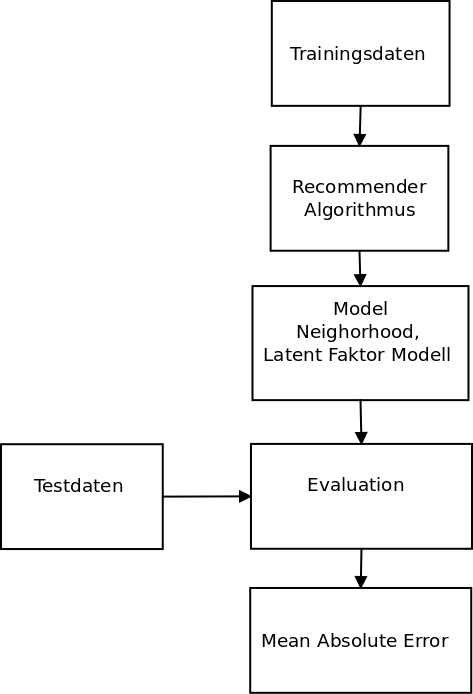
\includegraphics[width=0.5\textwidth]{evaluation}
  \caption{Collaborative Filtering Prozess}
\end{figure}

Die Bewertungen im Testset beinhalten den User $u$, das Item $i$ und die Bewertung pro Zeile. Mit dem berechneten Model muss der Recommender zu jedem $u$-$i$ Paar eine Bewertung vorhersagen. Diese Vorhersage vergleicht man mit dem tats"achlichen Bewertung aus dem Testset.

\subsection{Evaluationsmetrik}
\label{sec:evaluationmetrik}

Die Qualit"at des Recommendersystem kann mit Evaluationsmetriken "uberpr"uft werden. Evaluationsmetriken geben Auskunft dar"uber wie gut das Recommendersystem ist. Idealerweise kann ein Recommendersystem die Bewertung f"ur einen User und ein Item vorhersagen. Statistische Genauigkeitsmetriken geben an wie weit entfernt die Vorhersage vom tats"achlichen Wert ist. 

Es gibt verschieden Evaluationsmetriken. In diesem Projekt wurde der Mean Absolute Error als Metrik verwendet. MAE vergleicht die tats"achliche Bewertung eines User f"ur ein Item mit der Bewertung, die der Recommender berechnet hat. Man bildet die Differenz von Vorhersage und tats"achlicher Bewertung. Von der Differenz wird der Betrag berechnet. Schliesslich bestimmt man die mittlere Abweichung, indem man durch Anzahl Bewertungen $N$ im Testset teilt 

Der MAE ist wie folgt definiert \cite{sarwar01}:

\begin{equation}
  \label{eq:mae}
  MAE = \frac{\sum_{i+1}^N | p_i-q_i | }{N}
\end{equation}

Je tiefer der MAE, desto besser ist die Genauigkeit des Recommender.

Root Mean Sqaured Error und Correlation sind zwei weitere Metriken.

\section{Resultate}
\label{sec:results}

In diesem Abschnitt werden die Resultate der Evaluierung pr"asentiert.

Um die implementieren Techniken zu evaluieren, werden sie mit Baselinealgorithmen verglichen. 
Folgende Baselinealgorithmen wurden eingesetzt:

\begin{description}
\item[globaler Durchschnitt] Der Durchschnitt aller Ratings
\item[Item Durchschnitt] Der Durchschnitt aller Ratings f"ur ein Item
\item[User Durchschnitt] Der Durchschnitt aller Ratings die ein User vergeben hat
\end{description}

\begin{tikzpicture}
  \begin{axis}[
    xbar, xmin=0,
    width=12cm, enlarge y limits=0.5,
    symbolic y coords = {Global-AVG,Item-AVG,User-AVG,Useruser,Useruserp, Matrixfactorization},
    xlabel={MeanAbsoluteError},
    ytick = data,
    nodes near coords, nodes near coords align={horizontal},
    ]
    \addplot coordinates {(1.044,Global-AVG) (0.930,User-AVG) (0.872,Item-AVG) (0.857,Useruser) (0.8404,Useruserp) (0.76,Matrixfactorization)};
  \end{axis}
\end{tikzpicture}

Aus der Abbildung ist ersichtlich, dass der Fehler des Recommender bei Useruser am geringsten ist.

\section{Arbeitsspeicher Nutzung}
\label{sec:ram}

Bei einer Ratingmatrix r mit der Dimension von 1682 mal 943 konsumiert das Programm zu viel Arbeitsspeicher. Es werden 10GB angefordert. Profiling hat gezeigt die Fehler Berechnung viel Arbeitsspeicher konpsumiert.

\begin{equation}
  \label{eq:squareerror}
  \sum_{(u,i) \in \kappa} (r_{ui} - q_i^T p_u)^2
\end{equation}

$\kappa$ ist die Menge aller User-Item Paare, f"ur die ein Rating bekannt ist.

\bibliographystyle{plain}
\bibliography{a}
\end{document}